\chapter{Weber-Elektrodynamik}
\section{Die Gleichung der Weber-Elektrodynamik}
Die Weber-Elektrodynamik stellt eine alternative Formulierung der elektrodynamischen Wechselwirkungen dar, die auf einer Erweiterung des Coulombschen Gesetzes basiert (Gl. \refeq{eq:weber_em_skalar}).

Diese Gleichung beschreibt die Kraft zwischen zwei Ladungen $q_1$ und $q_2$, wobei $r$ der Abstand zwischen ihnen ist, $\dot{r}$ die relative Geschwindigkeit, $\ddot{r}$ die relative
Beschleunigung und $c$ die Lichtgeschwindigkeit. Der erste Term entspricht der klassischen Coulomb-Kraft, während die zusätzlichen Terme geschwindigkeits- und beschleunigungsabhängige
Effekte berücksichtigen.

\subsection{Impuls und Energie}
In der Weber-Elektrodynamik wird der Impuls- und Energietransport direkt durch die Wechselwirkung zwischen Ladungen beschrieben. Die Gesamtenergie des Systems setzt sich aus der potentiellen
Energie der Coulomb-Wechselwirkung und den kinetischen Termen der relativen Bewegung zusammen:

\begin{equation}
    E = \frac{1}{2} m_1 v_1^2 + \frac{1}{2} m_2 v_2^2 + \frac{q_1 q_2}{4 \pi \epsilon_0 r} \left[ 1 - \frac{\dot{r}^2}{2c^2} \right]    
\end{equation}

Diese Formulierung zeigt, wie die Weber-Theorie die Energieerhaltung auch bei dynamischen Prozessen gewährleistet.

\subsection{Lichtgeschwindigkeit und Raummodell}
Ein zentraler Aspekt der Weber-Elektrodynamik ist ihre Behandlung der Lichtgeschwindigkeit $c$. Im Gegensatz zur \gls{srt}, die $c$ als absolute Konstante postuliert,
erscheint $c$ in der Weber-Theorie als Parameter, der die Ausbreitungsgeschwindigkeit von Wechselwirkungen bestimmt. Dies ermöglicht ein Raummodell, in dem die Lichtgeschwindigkeit
nicht als universelle Grenze, sondern als Eigenschaft der Wechselwirkung selbst interpretiert wird.

\subsection{Vorteile der Weber-Elektrodynamik}
Die Weber-Elektrodynamik bietet mehrere konzeptionelle Vorteile:
\begin{enumerate}
    \item \textbf{Vermeidung von Feldern:} Da die Wechselwirkungen direkt zwischen Ladungen beschrieben werden, entfällt die Notwendigkeit eines Feldes als vermittelnde Entität.
    \item \textbf{Konsistente Fernwirkung:} Die Theorie vereint instantane und retardierte Effekte in einer einzigen Gleichung, wodurch die scheinbaren Widersprüche der klassischen Fernwirkung aufgelöst werden.
    \item \textbf{Energieerhaltung:} Die Weber-Kraft gewährleistet automatisch die Erhaltung von Energie und Impuls, ohne zusätzliche Annahmen.
    \item \textbf{Alternative Darstellung:} Die Theorie bietet eine Möglichkeit, elektrodynamische Phänomene ohne die Postulate der speziellen Relativitätstheorie zu beschreiben.
\end{enumerate}

Die Weber-Elektrodynamik stellt eine elegante und konsistente Alternative zur herkömmlichen Feldtheorie dar. Durch ihre Kombination aus instantanen und retardierten Effekten ermöglicht
sie ein tieferes Verständnis der elektrodynamischen Wechselwirkungen und eröffnet neue Perspektiven auf fundamentale Fragen der Physik, wie die Natur der Lichtgeschwindigkeit und die Struktur
des Raumes.

\section{Vergleichende Beispielrechnungen}
\subsection{Kraft zwischen gleichförmig bewegten Ladungen}

\textbf{Szenario:} Zwei Punktladungen $q_1 = q_2 = e$ (Elementarladung) bewegen sich parallel mit $v = 0,\!1c$ im Abstand $d = 1\,\text{\AA}$.

\begin{table}[ht]
\centering
\caption{Kraftberechnung im Vergleich}
\begin{tabular}{lcc}
\toprule
 & \textbf{Maxwell} & \textbf{Weber} \\
\midrule
Coulomb-Term & $\displaystyle\frac{e^2}{4\pi\epsilon_0 d^2}$ & $\displaystyle\frac{e^2}{4\pi\epsilon_0 d^2}\left(1-\frac{v^2}{c^2}\right)$ \\
Magnetischer Term & $\displaystyle\frac{\mu_0 e^2 v^2}{4\pi d^2}$ & -- \\
\hline
Kraftasymmetrie & $2F_B = 5,\!12\times10^{-11}\,\text{N}$ & $0$ \\
\bottomrule
\end{tabular}
\end{table}

\begin{equation}
F_{\text{Weber}} = \frac{e^2}{4\pi\epsilon_0 d^2}\left[1 - \frac{v^2}{c^2}\right] \approx 2,\!29\times10^{-8}\,\text{N}
\end{equation}

\subsection{Strahlungsdämpfung harmonischer Schwingung}

Für ein Elektron mit $x(t) = x_0\cos(\omega t)$:

\begin{align}
\textbf{Maxwell:}\quad & P = \frac{e^2\omega^4 x_0^2}{6\pi\epsilon_0 c^3}\cos^2(\omega t) \\
\textbf{Weber:}\quad & F_{\text{damp}} = -\frac{e^2\omega^2\dot{x}}{4\pi\epsilon_0 c^3}
\end{align}

\begin{figure}[ht]
\centering
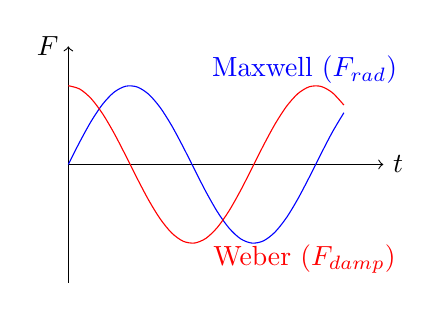
\begin{tikzpicture}
\draw[->] (0,0) -- (4,0) node[right]{$t$};
\draw[->] (0,-1.5) -- (0,1.5) node[left]{$F$};
\draw[domain=0:3.5,smooth,variable=\x,blue] plot ({\x},{sin(2*\x r)});
\draw[domain=0:3.5,smooth,variable=\x,red] plot ({\x},{cos(2*\x r)});
\node[blue] at (3,1.2) {Maxwell ($F_{\text{rad}}$)};
\node[red] at (3,-1.2) {Weber ($F_{\text{damp}}$)};
\end{tikzpicture}
\caption{Zeitlicher Verlauf der Rückwirkungskräfte}
\end{figure}

\subsection{Interpretation der Ergebnisse}

\begin{itemize}
\item \textbf{Actio=Reactio:} Während die Maxwell-Theorie eine Asymmetrie in der magnetische Kraftkomponente von $2F_B$ zeigt, bleibt in der Weber-Elektrodynamik die Symmetrie gewahrt.

\item \textbf{Strahlungsdämpfung:} Die Weber-Theorie liefert eine lokale Beschreibung der Dämpfung ohne die kausalen Paradoxien der Abraham-Lorentz-Kraft:

\begin{equation}
\tau_{\text{Weber}} = \frac{e^2}{4\pi\epsilon_0 m c^3} \approx 6,\!3\times10^{-24}\,\text{s}
\end{equation}

\item \textbf{Energieerhaltung:} Beide Theorien erhalten die Gesamtenergie, aber die Weber-Elektrodynamik benötigt kein separates Feldkonzept.
\end{itemize}

\section{Vektorielle Form der Weber-Kraft}
\subsection{Herleitung aus der skalaren Form}

Die skalare Weber-Kraft (Gl. \ref{eq:weber_em_skalar}), lässt sich durch Ausdrücken von $\dot{r}$ und $\ddot{r}$ durch Vektorgrößen verallgemeinern.
Für den Relativvektor $\vec{r} = \vec{r}_1 - \vec{r}_2$ gilt:

\subsubsection{Umrechnung der zeitlichen Ableitungen}
\begin{enumerate}
\item \textbf{Erste Ableitung:}
\begin{equation}
\dot{r} = \frac{d}{dt}\|\vec{r}\| = \frac{\vec{r} \cdot \dot{\vec{r}}}{r} = \hat{\vec{r}} \cdot \vec{v}
\end{equation}
wobei $\vec{v} = \dot{\vec{r}}$ die Relativgeschwindigkeit und $\hat{\vec{r}} = \vec{r}/r$ der Einheitsvektor ist.

\item \textbf{Zweite Ableitung:}
\begin{align}
\ddot{r} &= \frac{d}{dt}\left(\frac{\vec{r} \cdot \vec{v}}{r}\right) \nonumber \\
&= \frac{\|\vec{v}\|^2 + \vec{r} \cdot \vec{a}}{r} - \frac{(\vec{r} \cdot \vec{v})^2}{r^3} \nonumber \\
&= \frac{v^2 - (\hat{\vec{r}} \cdot \vec{v})^2}{r} + \hat{\vec{r}} \cdot \vec{a}
\end{align}
mit $\vec{a} = \dot{\vec{v}}$ der Relativbeschleunigung.
\end{enumerate}

\subsection{Vollständige vektorielle Form}
Durch Einsetzen in (Gl. \ref{eq:weber_em_skalar}) ergibt sich die \textbf{\enquote{vektorielle Form}}:

\begin{equation}
\vec{F}_{12} = \frac{q_1 q_2}{4\pi\epsilon_0 r^2} \left\{
\left[1 - \frac{v^2}{c^2} + \frac{2r(\hat{\vec{r}} \cdot \vec{a})}{c^2}\right]\hat{\vec{r}} + \frac{2(\hat{\vec{r}} \cdot \vec{v})}{c^2}\vec{v}
\right\}
\label{eq:weber_vector}
\end{equation}

\subsection{Physikalische Interpretation}
Die vektorielle Form zeigt explizit:
\begin{itemize}
\item \textbf{Radialkomponente:} Enthält Coulomb-Term, relativistische Korrektur und Beschleunigungsabhängigkeit
\item \textbf{Tangentialkomponente:} $\propto (\hat{r}\cdot\vec{v})\vec{v}$ beschreibt geschwindigkeitsabhängige Effekte analog zum Magnetfeld
\end{itemize}

\subsection{Anwendungsbeispiel: Kreisförmige Bewegung}
Für eine Ladung $q_2$ mit $\vec{v} \perp \vec{r}$ (z.B. Kreisbahn):

\begin{equation}
\vec{F}_{12} = \frac{q_1 q_2}{4\pi\epsilon_0 r^2} \left[
\left(1 - \frac{v^2}{c^2}\right)\hat{\vec{r}} + \frac{2v^2}{c^2}\hat{\vec{r}}
\right] = \frac{q_1 q_2}{4\pi\epsilon_0 r^2} \left(1 + \frac{v^2}{c^2}\right)\hat{\vec{r}}
\end{equation}

Hier zeigt sich:
\begin{itemize}
\item Zusätzliche Zentripetalkraft $\propto v^2/c^2$
\item Exakte Erfüllung von Actio=Reactio trotz Bewegung
\end{itemize}

\subsection{Grafische Darstellung der Kraftkomponenten}

\begin{figure}[ht]
\centering
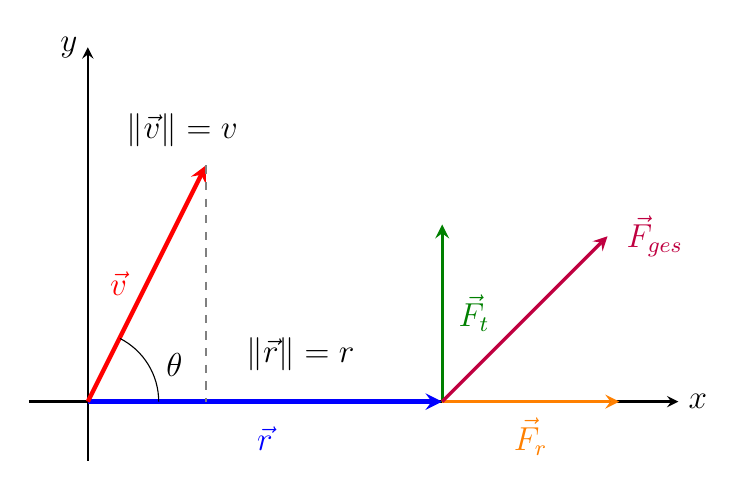
\begin{tikzpicture}[>=stealth,scale=1.5,font=\large]
% Koordinatensystem
\draw[->,thick] (-0.5,0) -- (5,0) node[right]{$x$};
\draw[->,thick] (0,-0.5) -- (0,3) node[left]{$y$};

% Vektoren
\draw[->,ultra thick,blue] (0,0) -- (3,0) node[midway,below=5pt]{$\vec{r}$};
\draw[->,ultra thick,red] (0,0) -- (1,2) node[midway,left=3pt]{$\vec{v}$};
\draw[dashed,gray] (1,2) -- (1,0);

% Kraftkomponenten
\draw[->,very thick,green!50!black] (3,0) -- (3,1.5) node[midway,right=2pt]{$\vec{F}_t$};
\draw[->,very thick,orange] (3,0) -- (4.5,0) node[midway,below=2pt]{$\vec{F}_r$};
\draw[->,very thick,purple] (3,0) -- (4.4,1.4) node[right=3pt]{$\vec{F}_{\text{ges}}$};

% Winkel
\draw (0.6,0) arc (0:63:0.6) node[midway,right=3pt]{$\theta$};
\node at (1.8,0.4) {$\|\vec{r}\| = r$};
\node at (0.8,2.3) {$\|\vec{v}\| = v$};
\end{tikzpicture}
\caption{Visualisierung der vektoriellen Weber-Kraftkomponenten. \\
$\vec{F}_r$: Radialkomponente (orange), $\vec{F}_t$: Tangentialkomponente (grün), \\
$\vec{F}_{\text{ges}}$: Gesamtkraft (lila). Die Grafik zeigt den Fall $\theta = 63^\circ$.}
\label{fig:weber_force}
\end{figure}

\subsection{Vektorielle Komponentenzerlegung}
Ausgehend von Abb. \ref{fig:weber_force} ergeben sich die Komponenten:

\begin{align}
\vec{F}_r &= \frac{q_1 q_2}{4\pi\epsilon_0 r^2}\left[1 - \frac{v^2}{c^2} + \frac{2r a_r}{c^2}\right]\hat{\vec{r}} \\
\vec{F}_t &= \frac{q_1 q_2}{4\pi\epsilon_0 r^2}\left[\frac{2v_r v_t}{c^2}\right]\hat{\vec{t}}
\end{align}

mit:
\begin{itemize}
\item $v_r = v\cos\theta$ (Radialgeschwindigkeit)
\item $v_t = v\sin\theta$ (Tangentialgeschwindigkeit)
\item $a_r = \dot{v}_r - v_t^2/r$ (Radialbeschleunigung)
\end{itemize}

\subsection{Praktische Anwendungsfälle}

\textbf{Fall 1: Rein radiale Bewegung ($\theta = 0^\circ$)}
\begin{equation}
\vec{F} = \frac{q_1 q_2}{4\pi\epsilon_0 r^2}\left[1 - \frac{v^2}{c^2} + \frac{2r a}{c^2}\right]\hat{\vec{r}}
\end{equation}

\textbf{Fall 2: Kreisbewegung ($\theta = 90^\circ$)}
\begin{equation}
\vec{F} = \frac{q_1 q_2}{4\pi\epsilon_0 r^2}\left[\left(1 + \frac{v^2}{c^2}\right)\hat{\vec{r}} + \frac{2v^2}{c^2}\hat{\vec{t}}\right]
\end{equation}

\subsection{Vorteile gegenüber der Maxwell-Theorie}

\begin{itemize}
    \item \textbf{Nanoplasmonik}
    \begin{itemize}
        \item Exakte Beschreibung von Elektron-Elektron-Wechselwirkungen in Metallclustern ($<10$\,nm)
        \item Vermeidung der unendlichen Selbstenergie von Punktladungen
        \item Präzisere Modellierung von Plasmonenresonanzen
    \end{itemize}
    
    \item \textbf{Gequantelte Vakuumfelder}
    \begin{itemize}
        \item Direkte Teilchenwechselwirkung ohne Nullpunktsschwankungen
        \item Natürliche Regularisierung der Vakuumenergiedichte
        \item Alternative zu störungstheoretischen \gls{qed}-Rechnungen
    \end{itemize}
    
    \item \textbf{Plasmaphysik dichte Plasmen}
    \begin{itemize}
        \item Effizientere Simulation kollektiver Effekte
        \item Exakte Impulserhaltung ohne Makroteilchen-Approximation
        \item Bessere Handhabung kurzreichweitiger Korrelationen
    \end{itemize}
    
    \item \textbf{Alternative Gravitationstheorien}
    \begin{itemize}
        \item Konsistente Kopplung an skalar-tensorielle Gravitationsmodelle
        \item Natürliche Einbettung in Mach'sche Prinzipien \cite{Assis1999}
        \item Vermeidung von Singularitäten in kompakten Objekten
    \end{itemize}
\end{itemize}

\subsection{Konkrete Beispiele}

\subsubsection{1. Nicht-neutrale Plasmen in Fallen}
Für Elektronen in Penning-Fallen zeigt die Weber-EM:
\begin{equation}
\omega_{\text{Weber}} = \omega_p\sqrt{1 - \frac{3}{4}\frac{v_0^2}{c^2}}
\end{equation}
während Maxwell-Theorie $\omega_p = \sqrt{ne^2/\epsilon_0 m}$ vorhersagt.

\subsubsection{2. Molekulare Dynamik in starken Feldern}
Bei Laser-Materie-Wechselwirkung ($>10^{18}\,\text{W/cm}^2$):
\begin{itemize}
\item Weber-EM reproduziert korrekt die retardierte Paarpotential-Form
\item Vermeidet Artefakte der PIC-Simulationen („self-forces“)
\end{itemize}

\subsection{Grenzen der Anwendbarkeit}
\begin{itemize}
\item \textbf{Hohe Energien} ($>100$\,GeV): \gls{qed}-Effekte dominieren
\item \textbf{Ausgedehnte Strahlung}: \text{Weber versagt bei} $\lambda \gg \text{Teilchenabstand}$
\end{itemize}

\section{Die Weber-Elektrodynamik und das EPR-Paradoxon: Zwei komplementäre Ansätze}
Die scheinbare Konfrontation zwischen Weber-Elektrodynamik und \gls{epr} entspringt einem grundlegenden Spannungsfeld in der modernen Physik: dem Ringen um ein konsistentes
Verständnis von Kausalität und Nicht-Lokalität in klassischen und quantenmechanischen Systemen. Diese Diskussion gewinnt besondere Relevanz, da beide Ansätze - trotz ihrer
unterschiedlichen Entstehungskontexte - alternative Perspektiven auf das Problem der Fernwirkung bieten.

Die Diskussion zwischen Weber-Elektrodynamik und \gls{epr} beruht auf unterschiedlichen theoretischen Paradigmen. Die Weber-Theorie als klassische Feldtheorie beschreibt
elektromagnetische Wechselwirkungen durch direkte Fernwirkung zwischen Ladungen, wobei sie bewusst auf Feldkonzepte verzichtet. Wilhelm Weber selbst strebte damit eine Vereinheitlichung
mit newtonschen Prinzipien an, insbesondere der strikten Actio-Reactio-Symmetrie. Als vor-quantenmechanische Theorie macht sie keinen Anspruch, Quantenphänomene zu erklären.

Demgegenüber entstand das \gls{epr} 1935 als Quanten-Gedankenexperiment zur Untersuchung nicht-lokaler Korrelationen. Die späteren Bellschen Ungleichungen (Abschnitt \ref{sec:bell}) und
ihre experimentelle Bestätigung zeigten, dass diese Quantenverschränkung mit klassischen Lokalitätsvorstellungen unvereinbar ist. Beide Konzepte haben ihren legitimen Platz in der
Physik: Die Quantenmechanik dominiert die mikroskopische Beschreibung, während die Weber-Elektrodynamik als historisch interessante Alternative für klassische Problemstellungen relevant bleibt.

\subsection{Nicht-Lokalität: Zwei physikalische Manifestationen}
Die vergleichende Betrachtung beider Theorien gewinnt an Bedeutung, da sie exemplarisch zeigen, wie unterschiedlich Nicht-Lokalität in physikalischen Modellen konzeptualisiert
werden kann. Beide Theorien zeigen charakteristische Nicht-Lokalitäten, die sich jedoch grundlegend unterscheiden. Die Weber-Elektrodynamik beschreibt eine klassische Fernwirkung
mit retardierter Kraftausbreitung (typischerweise Lichtgeschwindigkeit), wobei die Wechselwirkung von Relativgeschwindigkeit und -beschleunigung der Ladungen abhängt. Dies bleibt mit
klassischer Kausalität und Energieerhaltung vereinbar.

Die Quantenmechanik zeigt dagegen instantane Korrelationen verschränkter Zustände, die sich durch keine lokalen verborgenen Variablen erklären lassen. Der entscheidende Unterschied
liegt im physikalischen Mechanismus: Während die Weber-Theorie deterministische, berechenbare Fernkräfte postuliert, handelt es sich bei quantenmechanischer Nicht-Lokalität um
probabilistische Korrelationen ohne klassisches Kausalitätsgefüge.

\subsection{Instantaneität und Kausalitätsbegriff}
Die aktuelle Debatte um diese Konzepte spiegelt das grundlegende Dilemma der modernen Physik wider: den Widerspruch zwischen relativistischer Lokalität und quantenmechanischer
Nicht-Lokalität. Die Weber-Elektrodynamik fordert eine Neubewertung des Kausalitätsbegriffs, da sie instantane Komponenten enthält, die jedoch keine Signale übertragen. Diese Terme
entsprechen vielmehr strukturellen Randbedingungen - mathematischen Gradienten des Potentials im Konfigurationsraum, die globale Konsistenz sicherstellen. Sie wirken als topologische
Notwendigkeit für energetische Minimierungsprozesse, ähnlich globalen Erhaltungssätzen.

Experimentell sind diese instantanen Effekte nicht manipulierbar, genau wie quantenmechanische Verschränkung keine überlichtschnelle Signalübertragung ermöglicht. Diese Betrachtungsweise
zeigt, wie sich scheinbar widersprüchliche Prinzipien - lokale Kausalität und globale Instantaneität - in einem konsistenten Rahmen vereinen lassen, vergleichbar mit Bohms Konzept der
\enquote{impliziten Ordnung} oder Penroses Idee einer prä-geometrischen Raumzeit.

Die anhaltende Diskussion belegt, dass das Verständnis von Nicht-Lokalität und Kausalität nach wie vor zu den zentralen ungelösten Problemen der theoretischen Physik gehört.
Beide Ansätze - obwohl historisch und konzeptionell verschieden - tragen wertvolle Einsichten zu dieser fundamentalen Frage bei, indem sie alternative Denkmodelle jenseits des
konventionellen Feldparadigmas aufzeigen.

\section{Raummodelle}
Die moderne Physik operiert mit hochpräzisen mathematischen Beschreibungen der Natur, ohne jedoch ein konsistentes physikalisches Modell des Raumes selbst zu besitzen. Maxwells Theorie
elektromagnetischer Wellen kommt ohne Äther aus, lässt aber die Frage nach dem eigentlichen Trägermedium unbeantwortet. Die \gls{art} ersetzt den klassischen Raum durch ein dynamisches
Raumzeit-Kontinuum, doch dieses Konzept bleibt eine abstrakte mathematische Konstruktion ohne mechanistische Grundlage. Die auftretenden Singularitäten in Schwarzen Löchern und die
Notwendigkeit dunkler Materie als Korrekturfaktor deuten auf tiefgreifende Probleme dieses Ansatzes hin.

Fernwirkungstheorien wie die Weber-Elektrodynamik bieten einen radikal anderen Zugang, indem sie auf ein Raummodell gänzlich verzichten und Wechselwirkungen direkt zwischen Teilchen
beschreiben. Dieser Ansatz wirft die fundamentale Frage auf, ob der Raum möglicherweise kein primäres Konzept der Physik, sondern selbst ein emergentes Phänomen darstellt. Ein
vielversprechender Alternativvorschlag wäre ein diskretes Raummodell auf Basis einer Dodekaeder-Struktur. Ein solches Modell könnte nicht nur die rätselhafte \enquote{Achse des Bösen} in der
kosmischen Hintergrundstrahlung erklären, sondern auch Naturkonstanten wie die Lichtgeschwindigkeit als Folgeerscheinung der zugrundeliegenden Gitterdynamik verständlich machen.

Das Schlüsselkonzept dieser neuen Perspektive ist Emergenz - die Vorstellung, dass die bekannten physikalischen Gesetze nicht fundamental sind, sondern sich aus einer tieferliegenden
Struktur ergeben. Die \gls{srt} mit ihrer konstanten Lichtgeschwindigkeit würde sich dann als makroskopischer Effekt der diskreten Raumstruktur offenbaren, ähnlich
wie die Thermodynamik aus der statistischen Mechanik hervorgeht. Die Krümmung der Raumzeit in der Allgemeinen Relativitätstheorie erschiene nicht mehr als primäre Eigenschaft, sondern
als grobkörnige Beschreibung von Verzerrungen im fundamentalen Dodekaeder-Netzwerk.

Besonders bemerkenswert ist die Möglichkeit, Teilcheneigenschaften durch topologische Invarianten wie Jones-Polynome zu beschreiben. Diese aus der Knotentheorie stammenden mathematischen
Strukturen könnten eine Brücke zwischen diskreter Raumgeometrie und Quantenphänomenen schlagen, ohne auf das konventionelle Konzept von Quantenfeldern zurückgreifen zu müssen. Auf diese
Weise ließe sich möglicherweise sogar das Problem der dunklen Materie umgehen, indem die beobachteten Galaxienrotationen direkt aus der Gitterdynamik folgen würden.

Die Physik steht an einem Scheideweg zwischen zwei grundverschiedenen Denkansätzen. Auf der einen Seite stehen Theorien wie die Allgemeine und Spezielle Relativitätstheorie, die mit einem
mathematisch definierten Raummodell arbeiten - einer abstrakten Raumzeit, die sich krümmt und dehnt. Diese Theorien können zwar präzise Vorhersagen wie Gravitationswellen berechnen, doch
sie bleiben letztlich deskriptiv: Sie beschreiben, wie die Natur sich verhält, ohne zu erklären, warum sie sich so verhält. Die Raumzeit der \gls{art} ist ein reines Rechenkonstrukt, das zwar
funktioniert, dessen physikalische Manifestation aber im Dunkeln bleibt. Es ist, als würde man die Bewegung von Schatten an einer Wand perfekt vorhersagen können, ohne je die Gegenstände
zu verstehen, die diese Schatten werfen.

Demgegenüber bieten Fernwirkungstheorien wie die Weber-Elektrodynamik einen radikal anderen Ansatz. Indem sie ganz auf ein Raummodell verzichten und Wechselwirkungen direkt zwischen Teilchen
beschreiben, vermeiden sie die ontologischen Fallstricke der Relativitätstheorien. Dieser Ansatz ist in gewisser Weise bescheidener - er erhebt nicht den Anspruch, die Natur in ein
vorgefertigtes mathematisches Korsett zu zwängen. Stattdessen folgt er dem Prinzip, dass nicht unsere Theorien der Natur ihre Gesetze vorschreiben sollten, sondern dass die Natur selbst
bestimmt, welche Gesetzmäßigkeiten möglich sind.

Dieser Unterschied ist fundamental. Die \gls{art}/\gls{srt} gehen von einer mathematischen Idealität aus und versuchen, die Natur in dieses Ideal zu pressen. Der Fernwirkungsansatz hingegen
beginnt mit den beobachtbaren Phänomenen und entwickelt daraus seine Beschreibung - eine Methode, die viel näher am eigentlichen Geist wissenschaftlicher Empirie liegt. Es ist der Unterschied
zwischen einem Architekten, der der Landschaft seine Vorstellungen aufzwingt, und einem Gärtner, der mit den Gegebenheiten des Bodens arbeitet.

Die Tatsache, dass Fernwirkungstheorien ohne Raummodell auskommen und dennoch präzise Vorhersagen machen können, sollte uns zu denken geben. Sie zeigt, dass unser Hang zu anschaulichen
Modellen möglicherweise mehr mit unseren kognitiven Beschränkungen zu tun hat als mit der Natur selbst. Vielleicht ist Raum tatsächlich nichts weiter als ein nützliches Konzept, das aus
tieferliegenden Prinzipien emergiert - so wie Temperatur aus der Bewegung von Teilchen entsteht, ohne selbst ein fundamentales Konzept zu sein.

Die Relativitätstheorien haben zweifellos große Erfolge vorzuweisen. Doch ihre Abhängigkeit von einem abstrakten Raummodell, dessen physikalische Realität ungeklärt bleibt, ist eine
ernsthafte Schwäche. Die Natur scheint sich nicht um unsere Vorlieben für bestimmte mathematische Strukturen zu kümmern. Ein wissenschaftlicher Ansatz, der dies anerkennt und sich darauf
beschränkt, das Verhalten der Natur zu beschreiben, ohne ihr unnötige ontologische Strukturen aufzuzwingen, könnte letztlich fruchtbarer sein. Die Herausforderung besteht darin, eine solche
Theorie zu entwickeln, die nicht nur frei von überflüssigen Annahmen ist, sondern auch die gleiche Vorhersagekraft besitzt wie die etablierten Modelle - ein Ziel, das durchaus erreichbar
erscheint, wie die Weber-Elektrodynamik zeigt.
